\documentclass{article}
\usepackage{amsmath}
\usepackage{amssymb}
\usepackage[dvipsnames]{xcolor}
\usepackage{graphicx}
\usepackage{enumitem}
\usepackage{centernot}
\usepackage{multicol}
\usepackage{forest}
\usepackage{bm}
\usepackage[margin=1.2in]{geometry}
\definecolor{light-gray}{gray}{0.95}
\newcommand{\code}[1]{\colorbox{light-gray}{\texttt{#1}}}
\begin{document}

\title{Algorithms Midterm \#2}
\author{Ozaner Hansha}
\date{April 7, 2020}
\maketitle

\subsection*{Problem 1}
For the following question consider the following directed graph:
\begin{center}
  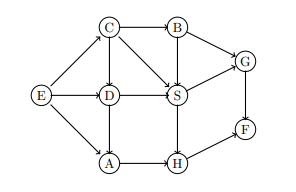
\includegraphics{graph.png}
\end{center}

\noindent\textbf{Part a:} Do a DFS starting at $C$, assuming vertices are to be considered in alphabetical order. List each vertex along with their discovery and finish times. Then classify each edge as a tree edge, back edge, forward edge, or cross edge.
\bigskip

\noindent\textbf{Solution:} The discovery and finish times for each vertex are given below (note that time starts at $t=1$):
\begin{center}
  \begin{tabular}{c|c|c}
        Vertex & Discovery Time & Finished Time \\
        \hline
        $A$ & $13$ & $14$\\
        $B$ & $2$ & $11$\\
        $C$ & $1$ & $16$\\
        $D$ & $12$ & $15$\\
        $E$ & $17$ & $18$\\
        $F$ & $4$ & $5$\\
        $G$ & $3$ & $6$\\
        $H$ & $8$ & $9$\\
        $S$ & $7$ & $10$
  \end{tabular}
\end{center}
\medskip

Note that after we finish node $C$ at time 16, we add the undiscovered node $E$ to the DFS stack at time 17. Recall that DFS returns a forest rather than just a tree. Each of the forest's edges is classified below:
\begin{center}
  \begin{tabular}{c|c|c|c}
        Tree Edges & Forward Edges & Cross Edges & Backward Edges \\
        \hline
        $(C,B),(C,D),(B,G),$ & $(C,S)$ & $(D,S),(S,G),(H,F),$\\
        $(B,S),(D,A),(G,F),$ & & $(A,H),(E,A),(E,C),$\\
        $(S,H)$ & & $(E,D)$
  \end{tabular}
\end{center}

\noindent\textbf{Part b:} Use the DFS from part a to do a topological sort on this graph. List the vertices on a line in topological sorted order.
\bigskip

\noindent\textbf{Solution:} Recall that performing a topological sort on a DAG, of which the above graph is due to not having any back edges, is equivalent to listing the finish times of of DFS in reverse order. Thus, our topological sort returns the following ordered list of vertices:

$$E,C,D,A,B,S,H,G,F$$

\noindent\textbf{Part c:} Identify the strongly connected components (SCCs) of the graph. Suppose now we switch the direction of the edges $(D,A)$ and $(E,D)$, what are the SCCs of the new graph?
\bigskip

\noindent\textbf{Solution:} Note that since the original graph was a DAG, every vertex is itself an SCC (every SCC is denoted by a blue box):
\begin{center}
  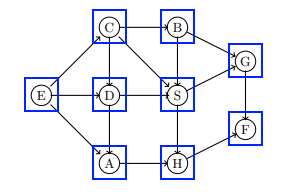
\includegraphics{graphSCC.png}
\end{center}

In the case of the modified graph, the SCCs are given by:
\begin{center}
  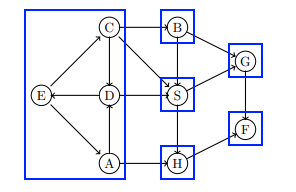
\includegraphics{graph2SCC.png}
\end{center}

\subsection*{Problem 2}
\noindent\textbf{Problem:} Suppose $n$ people attend a party and some shake hands with others. Prove there are at least two people who have shaken hands with the same number of people.
\bigskip

\noindent\textbf{Solution:} Consider a function $f(x)$ that returns the number of people the $x$th person at the party has shaken hands with. The domain of the $f$ is the integer interval $[1..n]$. The range is any number from 0 to $n-1$, since a person can shake anywhere from no hands to every other person's hands.

However, note that $f(i)=n-1$ and $f(j)=0$ are mutually exclusive for any $i$ and $j$. This is because if a person $i$ has shaken every other person's hands, there can be no person $j$ who has shaken no hands as $j$ would have at least shaken $i$'s hand. As such, no matter how the hand shaking takes place, $f$ can only output $n-1$ different values at most. Since there are $n$ possible inputs (i.e. $n$ people) the pigeonhole-principle tells us that that $f(i)=f(j)$ for some $i$ and $j$ (i.e. at least 2 people must have shaken hands the same number of times).

\subsection*{Problem 3}
\noindent\textbf{Problem:} Suppose in the process of computing the MST of a graph with 17 vertices via Kruskal’s algorithm we have obtained connected components having sizes 2,4,5,6. Using weighted-union, give all possible scenarios as well the minimum and maximum number of possible operations needed to get an MST.

(An operation is changing a link. For example, if the component with 2 elements gets added to the component with 4 elements, we change two links for the smaller set plus linking the head of shorter to the tail of
the longer, for a total of 3 operations.)
\bigskip

\noindent\textbf{Solution:} Below is a tree detailing all 18 possible ways these 4 connected components could form an MST.
\medskip

\hspace*{-1.2in}
\scalebox{.85}{
\begin{forest}
  for tree={l sep+=.8cm,s sep+=.5cm,shape=rectangle, rounded corners,
      draw, align=center,
      top color=white, bottom color=white}
  [{$\{2,4,5,6\}$\\0 ops}
    [{$\{5,6,6\}$\\3 ops},edge label={node[midway,left]{$2\cup4$}}
      [{$\{6,11\}$\\9 ops},edge label={node[midway,left]{$5\cup6$}}
        [{$\{17\}$\\16 ops},edge label={node[midway,left]{$6\cup11$}}]
      ]
      [{$\{6,11\}$\\9 ops},edge label={node[midway,midway]{$5\cup6$}}
        [{$\{17\}$\\16 ops},edge label={node[midway,left]{$6\cup11$}}]
      ]
      [{$\{5,12\}$\\10 ops},edge label={node[midway,right]{$6\cup6$}}
        [{$\{17\}$\\16 ops},edge label={node[midway,left]{$5\cup12$}}]
      ]
    ]
    [{},edge label={node[midway,midway]{$2\cup5$}}[[[[{$\{4,6,7\}$\\3 ops}
      [{$\{7,10\}$\\8 ops},edge label={node[midway,left]{$4\cup6$}}
        [{$\{17\}$\\16 ops},edge label={node[midway,left]{$10\cup7$}}]
      ]
      [{$\{6,11\}$\\8 ops},edge label={node[midway,midway]{$4\cup7$}}
        [{$\{17\}$\\15 ops},edge label={node[midway,left]{$6\cup11$}}]
      ]
      [{$\{4,13\}$\\10 ops},edge label={node[midway,right]{$6\cup7$}}
        [{$\{17\}$\\15 ops},edge label={node[midway,left]{$4\cup13$}}]
      ]
    ]]]]]
    [{$\{4,5,8\}$\\3 ops},edge label={node[midway,midway]{$2\cup6$}}
      [{$\{8,9\}$\\8 ops},edge label={node[midway,left]{$4\cup5$}}
        [{$\{17\}$\\17 ops},edge label={node[midway,left]{$8\cup9$}}]
      ]
      [{$\{5,12\}$\\8 ops},edge label={node[midway,midway]{$4\cup8$}}
        [{$\{17\}$\\14 ops},edge label={node[midway,left]{$5\cup12$}}]
      ]
      [{$\{4,13\}$\\9 ops},edge label={node[midway,right]{$5\cup8$}}
        [{$\{17\}$\\14 ops},edge label={node[midway,left]{$4\cup13$}}]
      ]
    ]
    [{},edge label={node[midway,midway]{$4\cup5$}}[[[[{$\{2,6,9\}$\\5 ops}
      [{$\{8,9\}$\\8 ops},edge label={node[midway,left]{$2\cup6$}}
        [{$\{17\}$\\17 ops},edge label={node[midway,left]{$8\cup9$}}]
      ]
      [{$\{6,11\}$\\8 ops},edge label={node[midway,midway]{$2\cup9$}}
        [{$\{17\}$\\15 ops},edge label={node[midway,left]{$6\cup11$}}]
      ]
      [{$\{9,15\}$\\12 ops},edge label={node[midway,right]{$6\cup9$}}
        [{$\{17\}$\\15 ops},edge label={node[midway,left]{$2\cup15$}}]
      ]
    ]]]]]
    [{$\{2,5,10\}$\\5 ops},edge label={node[midway,midway]{$4\cup6$}}
      [{$\{7,10\}$\\8 ops},edge label={node[midway,left]{$2\cup5$}}
        [{$\{17\}$\\16 ops},edge label={node[midway,left]{$7\cup10$}}]
      ]
      [{$\{5,12\}$\\8 ops},edge label={node[midway,midway]{$2\cup10$}}
        [{$\{17\}$\\14 ops},edge label={node[midway,left]{$5\cup12$}}]
      ]
      [{$\{2,15\}$\\11 ops},edge label={node[midway,right]{$5\cup10$}}
        [{$\{17\}$\\14 ops},edge label={node[midway,left]{$2\cup15$}}]
      ]
    ]
    [{},edge label={node[midway,right]{$5\cup6$}}[[[[{$\{2,4,11\}$\\6 ops}
      [{$\{6,11\}$\\9 ops},edge label={node[midway,left]{$2\cup4$}}
        [{$\{17\}$\\16 ops},edge label={node[midway,left]{$6\cup11$}}]
      ]
      [{$\{4,13\}$\\9 ops},edge label={node[midway,midway]{$2\cup11$}}
        [{$\{17\}$\\14 ops},edge label={node[midway,left]{$4\cup13$}}]
      ]
      [{$\{2,15\}$\\11 ops},edge label={node[midway,right]{$4\cup11$}}
        [{$\{17\}$\\14 ops},edge label={node[midway,left]{$2\cup15$}}]
      ]
    ]]]]]
  ]  
\end{forest}}
\medskip

As we can see, the min and max number of operations combining these sets would take are 14 and 17 respectively.

\subsection*{Problem 4}
\noindent\textbf{Part a:} Compute the MST of the following graph using Kruskal’s algorithm. Show the order of the selected edges as well as the sets formed. If there is a tie use alphabetical ordering.
\begin{center}
  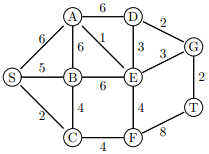
\includegraphics{graph4a.png}
\end{center}
\bigskip

\noindent\textbf{Solution:} The sets of spanned vertices and corresponding selected edge are given in the following table:
\begin{center}
\begin{tabular}{c|c|c|c}
  \textbf{Time} & \textbf{Selected} & &\\
  \textbf{Step} & \textbf{Edge} & \textbf{Added?} & \textbf{Sets of Spanned Vertices}\\
  \hline
  0 & - & - & $\{A\},\{B\},\{C\},\{D\},\{E\},\{F\},\{G\},\{H\},\{S\}$\\
  \hline
  1 & $(A,S)$ & Yes & $\{A,S\},\{B\},\{C\},\{D\},\{E\},\{F\},\{G\},\{H\}$\\
  \hline
  2 & $(G,H)$ & Yes & $\{A,S\},\{B\},\{C\},\{D\},\{E\},\{F\},\{G,H\}$\\
  \hline
  3 & $(A,B)$ & Yes & $\{A,B,S\},\{C\},\{D\},\{E\},\{F\},\{G,H\}$\\
  \hline
  4 & $(B,S)$ & No &  $\{A,B,S\},\{C\},\{D\},\{E\},\{F\},\{G,H\}$\\
  \hline
  5 & $(C,F)$ & Yes & $\{A,B,S\},\{C,F\},\{D\},\{E\},\{G,H\}$\\
  \hline
  6 & $(B,C)$ & Yes & $\{A,B,C,F,S\},\{D\},\{E\},\{G,H\}$\\
  \hline
  7 & $(B,E)$ & Yes & $\{A,B,C,E,F,S\},\{D\},\{G,H\}$\\
  \hline
  8 & $(A,E)$ & No &  $\{A,B,C,E,F,S\},\{D\},\{G,H\}$\\
  \hline
  9 & $(C,S)$ & No &  $\{A,B,C,E,F,S\},\{D\},\{G,H\}$\\
  \hline
  10 & $(D,E)$ & Yes & $\{A,B,C,D,E,F,S\},\{G,H\}$\\
  \hline
  11 & $(D,G)$ & Yes & $\{A,B,C,D,E,F,G,H,S\}$
\end{tabular}
\end{center}
\smallskip

Once $(D,G)$ is added to the spanning tree, our sets have all been combined and our MST is complete:
\begin{center}
  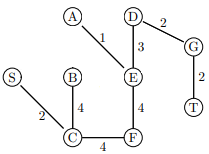
\includegraphics{graph4aMST.png}
\end{center}
\newpage

\noindent\textbf{Part b:} Compute the MST of the following graph using Prim's algorithm. Start at $S$ and give the order of the selected edges.
\begin{center}
  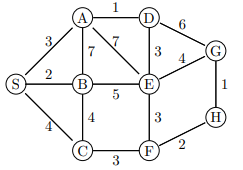
\includegraphics{graph4b.png}
\end{center}
\bigskip

\noindent\textbf{Solution:} Running Prim's algorithm starting at $S$ nets us:
\begin{center}
\begin{tabular}{c|c|c}
  \textbf{Order} & \textbf{Edge} & \textbf{Spanned Vertices}\\
  \hline
  1 & $(B,S)$ & $B,S$\\
  \hline
  2 & $(A,S)$ & $A,B,S$\\
  \hline
  3 & $(A,D)$ & $A,B,D,S$\\
  \hline
  4 & $(D,E)$ & $A,B,D,E,S$\\
  \hline
  5 & $(E,F)$ & $A,B,D,E,F,S$\\
  \hline
  6 & $(F,H)$ & $A,B,D,E,F,H,S$\\
  \hline
  7 & $(H,G)$ & $A,B,D,E,F,G,H,S$\\
  \hline
  8 & $(C,F)$ & $A,B,C,D,E,F,G,H,S$
\end{tabular}
\end{center}
\smallskip

Once $(C,F)$ is added to the spanning tree, all vertices have been spanned and our MST is complete:
\begin{center}
  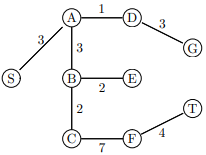
\includegraphics{graph4bMST.png}
\end{center}
\newpage

\noindent\textbf{Part c:} Using Dijkstra’s algorithm find the shortest path from S to all other vertices. Show the complete update history of each vertex $v$, starting with infinity as the value of $d(v), v\not= S$, and finishing with the length of the shortest path.
\begin{center}
  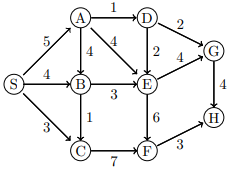
\includegraphics{graph4c.png}
\end{center}
\bigskip

\noindent\textbf{Solution:} Each iteration of Dijkstra’s algorithm is given below:
\bigskip

\hspace*{-0.4in}
\begin{tabular}{c|c|c|c|c|c|c|c|c|c}
  \textbf{Iteration} & $\bm{S}$ & $\bm{A}$ & $\bm{B}$ & $\bm{C}$ & $\bm{D}$ & $\bm{E}$ & $\bm{F}$ & $\bm{G}$ & $\bm{H}$\\\hline
  0 & 0, Null & $\infty$, Null & $\infty$, Null & $\infty$, Null & $\infty$, Null & $\infty$, Null & $\infty$, Null & $\infty$, Null & $\infty$, Null\\\hline
  1 & \textbf{0, Null} & 5, $S$ & 4, $S$ & 3, $S$ & $\infty$, Null & $\infty$, Null & $\infty$, Null & $\infty$, Null & $\infty$, Null\\\hline
  2 & - & 5, $S$ & 4, $S$ & $\bm{3, S}$ & $\infty$, Null & $\infty$, Null & 10, $C$ & $\infty$, Null & $\infty$, Null\\\hline
  3 & - & 5, $S$ & $\bm{4, S}$ & - & $\infty$, Null & 7, $B$ & 10, $C$ & $\infty$, Null & $\infty$, Null\\\hline
  4 & - & $\bm{5, S}$ & - & - & 6, $A$ & 7, $B$ & 10, $C$ & $\infty$, Null & $\infty$, Null\\\hline
  5 & - & - & - & - & $\bm{6, A}$ & 7, $B$ & 10, $C$ & 8, $D$ & $\infty$, Null\\\hline
  6 & - & - & - & - & - & $\bm{7, B}$ & 10, $C$ & 8, $D$ & $\infty$, Null\\\hline
  7 & - & - & - & - & - & - & 10, $C$ & $\bm{8, D}$ & 12, $G$\\\hline
  8 & - & - & - & - & - & - & $\bm{10, C}$ & - & 12, $G$\\\hline
  9 & - & - & - & - & - & - & - & - & $\bm{12, G}$
\end{tabular}
\bigskip

From this table we can construct the following shortest path tree with root $S$:
\begin{center}
  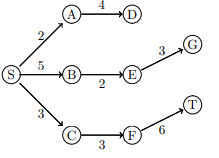
\includegraphics{graph4cSPT.png}
\end{center}
\newpage

\subsection*{Problem 5}
\noindent\textbf{Problem:} Write the system of linear inequalities corresponding to the following graph, then use the approach based on Bellman-Ford to find a solution to the system of inequalities using inspection or prove there is no solution. Do the same when the weight of the edge $(v_6, v_4)$ is changed to $-5$.
\begin{center}
  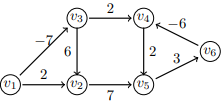
\includegraphics{inequalities.png}
\end{center}
\bigskip

\noindent\textbf{Solution:} The corresponding inequalities are given by:
\begin{alignat*}{4}
  x_3-x_1&\le-7  &\qquad  x_2-x_1&\le2  &\qquad  x_2-x_3&\le6 &\qquad x_5-x_2&\le7\\
  x_4-x_3&\le2  &  x_5-x_4&\le2 &  x_4-x_6&\le-6 & x_6-x_5&\le3\\
\end{alignat*}

Upon inspection, we note that there is a negative cycle $(v_4,v_5,v_6)$ summing to -1. As a result, there is no solution to the corresponding system of inequalities.

Changing $(v_6,v_4)$, and its corresponding inequality, to have a weight of -5, we no longer have a negative cycle and produce the following iteration of Bellman-Ford with the additional node $v_0$:
\begin{center}
  \begin{tabular}{c|c|c|c|c|c|c|c}
    \textbf{Iteration} & $\bm{v_0}$ & $\bm{v_1}$ & $\bm{v_2}$ & $\bm{v_3}$ & $\bm{v_4}$ & $\bm{v_5}$ & $\bm{v_6}$\\
    \hline
    0 & 0, Null & $\infty$, Null & $\infty$, Null & $\infty$, Null & $\infty$, Null & $\infty$, Null & $\infty$, Null\\
    \hline
    1 & 0, Null & 0, $v_0$ & 0, $v_0$ & -7, $v_1$ & -5, $v_3$ & -3, $v_4$ & 0, $v_0$\\
    \hline
    2 & 0, Null & 0, $v_0$ & -1, $v_3$ & -7, $v_1$ & -5, $v_3$ & -3, $v_4$ & 0, $v_0$\\
    \hline
    3 & 0, Null & 0, $v_0$ & -1, $v_3$ & -7, $v_1$ & -5, $v_3$ & -3, $v_4$ & 0, $v_0$\\
    \hline
    4 & 0, Null & 0, $v_0$ & -1, $v_3$ & -7, $v_1$ & -5, $v_3$ & -3, $v_4$ & 0, $v_0$\\
    \hline
    5 & 0, Null & 0, $v_0$ & -1, $v_3$ & -7, $v_1$ & -5, $v_3$ & -3, $v_4$ & 0, $v_0$\\
    \hline
    6 & 0, Null & 0, $v_0$ & -1, $v_3$ & -7, $v_1$ & -5, $v_3$ & -3, $v_4$ & 0, $v_0$
  \end{tabular}
\end{center}

After $7-1=6$ iterations we can be sure that we have our solution:
\begin{alignat*}{3}
  x_1  & = 0  &\qquad  x_2 &  = -1  &\qquad  x_3  & = -7\\
  x_4  & = -5  &  x_5 & = -3 &  x_6  & = 0\\
\end{alignat*}

\subsection*{Problem 6}
\noindent\textbf{Part a:} Assume $G = (V, E)$ is an undirected connected graph consisting of a spanning tree plus one more edge. The edges have weights. Describe an efficient algorithm for computing MST and its complexity in terms of $n=|V|$.
\bigskip

\noindent\textbf{Solution:} Since the graph was a spanning tree before the extra edge was added, there must be one cycle in the graph. Our goal is to find this cycle and remove the edge in that cycle with the highest weight. Since we can only remove one edge before the graph is a spanning tree, removing the highest one ensures it is a MST. We do this by performing the following algorithm:

Perform DFS on any of the nodes, making sure to store each visited edge in order on a stack as well as to mark each node visited when discovered. The search will eventually reach a node that has been visited before (because it is connected and must have a cycle as previously mentioned). When this happens we store that node as \code{twiceNode} and store the edge that led to it as \code{largestEdge}. From this point on we abandon the DFS and instead backtrack through the edge stack we have stored, making sure to compare each edge with \code{largestEdge} and replacing it if larger. We stop this backtracking once we reach \code{twiceNode} again.

At this point our algorithm is complete. We now simply remove \code{largestEdge} (which is the largest edge in the cycle) from the given graph and we are left with the MST.

In terms of complexity, in the worst case the above algorithm will move through all edges twice (once forward and once backwards) as well as encountering one vertex twice and the rest once. The complexity of encountering an edge or vertex is constant and so too is the complexity of removing the largest edge at the end of the algorithm. This leaves us with $k_1|E|+k_1(|V|+1)$ operations which is $O(|E|+|V|)$. However, note that since this graph is a spanning tree (which all have exactly $|V|-1$ edges) plus an extra edge, we have that there are $|V|-1+1=|V|$ edges on this graph. And so the complexity reduces to: $O(|E|+|V|)=O(|V|+|V|)=O(|V|)=O(n)$.
\bigskip

\noindent\textbf{Part b:} Let $G=(V,E)$ be an undirected complete graph with n vertices. Suppose after we have computed the MST of $G$ we realize that we missed one of the nodes so that $G$ is actually a complete graph with $n+1$ nodes. Describe an efficient algorithm for computing the MST of the augmented graph.
\bigskip

\noindent\textbf{Solution:} Given an MST of the graph \textit{without} the new node, we only need to add the edge with the smallest weight that connects to the new node. This will result in an MST of the augmented graph.

In the worst case, this new node will be connected to every other node (i.e. have $n$ edges). As such, it will take a selection algorithm $O(n)$ time to find the (not necessarily unique) smallest edge and constant time to add it to the old MST, resulting in a total complexity of $O(n)$.
\bigskip

\noindent\textbf{Part c:} Suppose $G=(V,E)$, where $n=|V|$ and $m=|E|$, is an edge weighted graph where the edge weights are distinct (no two edges have the same weight). Prove the MST of $G$ is unique.
\bigskip

\noindent\textbf{Solution:} Suppose there are two distinct MSTs $A$ and $B$. Let $e$ be the smallest edge in $A\Delta B$ (i.e. the smallest edge not shared by $A$ and $B$). W.l.o.g. we can say $e\in A$.

Now call $e=(P,Q)$. Since $e\not\in B$, $B$ must contain some other path from $P$ to $Q$ since it is a spanning tree. As such, the union $B\cup\{e\}$ must contain a cycle since it contains two paths from $P$ to $Q$. Note that if all the edges that were part of that cycle were in $A$, then $A$ would also have a cycle which violates its definition as an MST. As such, there must be at least one edge $f\in B$ such that it is part of that cycle but not in $A$.

Since $f\in A\Delta B$ we have, by definition, that $w(e)<w(f)$ since $e$ is the minimum edge in $A\Delta B$ and each edge has a distinct weight. As such, if we create a new graph $C=B\cup\{e\}\setminus\{f\}$, we find that it too is a spanning tree (as the removal of $f$ removes the cycle). However, you'll note that $C$ has strictly smaller total weight than $B$, since $w(e)<w(f)$. This contradicts our initial assumption that there are distinct minimum spanning trees $A$ and $B$, thus that assumption was false and there is only one unique MST.

\subsection*{Problem 7}
\noindent\textbf{Problem:} Are the following statements true or false?
\begin{enumerate}[label=\alph*)]
  \item  In an undirected graph the sum of the degrees of vertices is always twice the number of edges.
  \item We can use BFS to decide if a graph is bipartite.
  \item Given a complete graph on $n$ nodes, the number of cycles with at most 4 vertices is $O(2^n)$.
  \item We can use any minimum spanning tree algorithm to compute the maximum spanning tree, i.e. a spanning tree where the sum of the weights of its edges is maximum.
\end{enumerate}
\bigskip

\noindent\textbf{Solution:}
\begin{enumerate}[label=\alph*)]
  \item True
  \item True
  \item False
  \item True
\end{enumerate}

\end{document}